\documentclass[tikz,border=10pt]{standalone}
\usepackage{pgfplots}
\pgfplotsset{compat=1.18}

\begin{document}
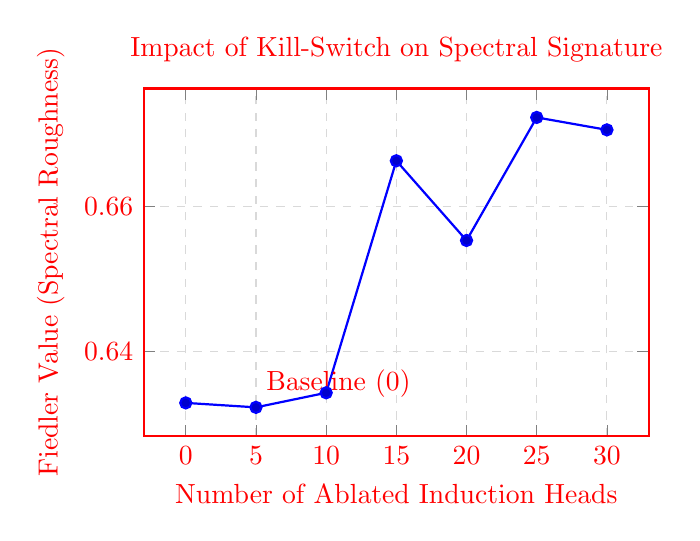
\begin{tikzpicture}
\pgfplotstableread[row sep=newline, col sep=comma]{
k,fiedler
0,0.6328332462906596
5,0.6322165499991812
10,0.6342318059806336
15,0.6663456141674106
20,0.6553160171436686
25,0.6723485586425901
30,0.6706259292888045

}\mydata

\begin{axis}[
    width=8cm, height=6cm,
    xlabel={Number of Ablated Induction Heads},
    ylabel={Fiedler Value (Spectral Roughness)},
    title={Impact of Kill-Switch on Spectral Signature},
    grid=major,
    grid style={dashed, gray!30},
    mark=*,
    mark options={fill=red},
    thick,
    red
]
\addplot table [x=k, y=fiedler] {\mydata};
\node[anchor=south west] at (axis cs: 5, 0.6322165499991812) {Baseline (0)};
\end{axis}
\end{tikzpicture}
\end{document}
